\documentclass[reqno]{amsart}
\usepackage{fancyhdr}
\usepackage{amsmath}
\usepackage{amssymb}
\usepackage{pifont}
\usepackage{booktabs}
\usepackage{subcaption}
\usepackage{graphicx}
\usepackage{verbatim}
\usepackage{hyperref}


\pagestyle{fancy}
\chead{2/4/22}
\rhead{Jackson Dougherty}
\renewcommand{\headrulewidth}{0.4pt}
\renewcommand{\footrulewidth}{0.4pt}

\hypersetup{
    colorlinks=true,     
    urlcolor=blue,
    }

\begin{document}
\section*{Riddler 2-4-22}
\section*{Jackson Dougherty}

\section{Riddler Express}

\subsection*{Problem}

An online quiz asks which three actors from the original "Scream" movie had returned for the fifth installment of the franchise. The quiz offers five choices:
\begin{itemize}
	\item Courtenay Cox
	\item David Arquette
	\item Halle Berry
	\item Neve Campbell
	\item Tom Holland
\end{itemize}

Suppose you have no idea of the correct three. IF you were to randomly choose three of the five actors, what is the probability that you would get at least two right?

\subsection*{Solution}

There are only $\binom{5}{3}=10$ possible guesses, so we can just enumerate them all. We abbreviate by the first initial of the star and mark whether we have two right in the following table:

\begin{table}[h]
\begin{tabular}{cccccc}\toprule
C & D & H & N & T & 2 right?\\\midrule
Y & Y & Y &  &  & \ding{51} \\
Y & Y &  & Y &  & \ding{51} \\
Y & Y &  &  & Y & \ding{51} \\
Y &  & Y & Y &  & \ding{51} \\
Y &  & Y &  & Y & \ding{55} \\
Y &  &  & Y & Y & \ding{51} \\
 & Y & Y & Y &  & \ding{51} \\
 & Y & Y &  & Y & \ding{55} \\
 & Y &  & Y & Y & \ding{51} \\
 &  & Y & Y & Y & \ding{55} \\\bottomrule
\end{tabular}
\end{table}

Comparing the number of guesses with two of the three stars to the total number of possible guesses, we have a 70\% change of getting at least two right. 

Reasoning slightly less directly, we observe that failing to get at least two right implies only getting one actor of the three correct. Since there are two incorrect and three correct actor choices, we need both incorrect actors in our guess, leaving one incorrect guess per returning actor.  

\section{Riddler Classic}

\subsection*{Problem}

A light source emits vertically polarized light, but we want horizontally polarized light. When light passes through a linear polarizer, the light becomes polarized to the axis of the polarizer, but its electric field vector is projected onto the polarizer axis. 

Concretely, if the angle between the polarizer and the incoming light's polarization axis is $\theta$, then the outgoing light's electric field $E_0$ can be written in terms of the incoming electric field $E_i$,
\begin{align*}
E_o = E_i \cos\theta
\end{align*} 

From this relationship, we cannot take the vertically polarized light to horizontal with only a single polarizer, for $\theta=\pi/2 \mapsto E_o=0$. Figure $\ref{fig:polarizers}$ shows how inserting intermediate polarizers will result in horizontally polarized light. 

However, inserting additional polarizers has a cost, since each polarizer only allows 99\% of the incoming electric field to pass through. Given a supply of polarizers, what is the optimal number of polarizers to create the largest horizontal electric field for outgoing light?

\begin{figure}[h]
	\centering
	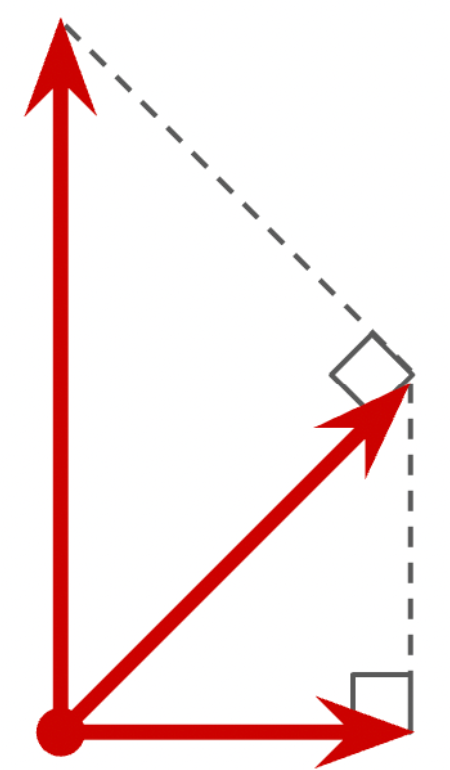
\includegraphics[scale = 0.5]{Polarizers.png}
	\caption{Placing an intermediate polarizer between the incoming vertically polarized light and a final, horizontal polarizer results in a nonzero horizontal electric field. The component relationship of incoming and outgoing electric field vectors is also evident from the shown triangles.}
	\label{fig:polarizers}
\end{figure}

\subsection*{Solution}

Given a setup of $N$ polarizers, we can describe the angle $\theta_i$ between the $i$th polarizer and the horizontal axis. We also define $\theta_0=\pi/2$ and $\theta_N=0$, since the incoming light is vertical and the final polarizer must be horizontal. As noted in the problem statement, we must have $N>1$ for any nonzero horizontal component to survive.

With this notation, we can write the final electric field for $N$ polarizers as a function of the $N-1$ free polarizer angles:
\begin{align*}
E_N(\theta_1, \theta_2, \ldots, \theta_{N-1}) &= \prod_{i=1}^{N} (0.99)\cos\left(\theta_i-\theta_{i-1}\right)\\
&= (0.99)^N \left(\prod_{i=1}^{N} \cos\left(\theta_i-\theta_{i-1}\right)\right)
\end{align*}

There are a two main components to the solution. We wish to determine the optimal configuration of the $N$ polarizers, since a known configuration allows us to write an expression for the surviving electric field. Then, we can find the value of $N$ that maximizes this value. 

We claim that evenly spacing the polarizers maximizes the final electric field. This claim is clear for $N=2$. In that case, the electric field is simply
\begin{align*}
E_2(\theta_1) &= (0.99)^2 \cos(\pi/2-\theta_1)\cos(\theta_1-0),
\end{align*}
which is maximized for $\theta=\pi/4$. 

The general case can be suggested by a perturbation from the evenly spaced arrangement. Any perturbation would take the form of a deviation $\delta$ that affects two terms in the product, 
\begin{align*}
\cos(\pi/2N + \delta)\cos(\pi/2N-\delta).
\end{align*}  
Series expansion about $\delta=0$ shows a negative $2$nd order term in the perturbation $\delta$.

With this understanding, the outgoing electric field for $N$ polarizers becomes 
\begin{align*}
E_N = (0.99)^N \cos^N\left(\frac{\pi}{2N}\right)
\end{align*}

The portion involving $\cos^N(\pi/2N)$ has the expected behavior that its limit is $1$ as $N\rightarrow \infty$. With infinite polarizers and no absorption or reflection, each polarizer would lose a negligible portion of the electric field. 

With the 1\% reflection, the maximum horizontal field occurs for $N=11$. With 11 polarizers, the horizontal electric field is approximately $0.8$ times the original vertical electric field. 




\end{document}